\documentclass[12pt,a4paper]{article}

% Packages
\usepackage[margin=1in]{geometry}
\usepackage{graphicx}
\graphicspath{{./figures/}}
\usepackage{amsmath}
\usepackage{booktabs}
\usepackage{hyperref}
\usepackage{xcolor}
\usepackage{listings}
\usepackage{enumitem}
\usepackage{titlesec}
\usepackage{fancyhdr}
\usepackage{caption}
\usepackage{array}
\usepackage{parskip}
\usepackage[section]{placeins}

% Header/Footer
\pagestyle{fancy}
\fancyhf{}
\rhead{TCP-Fusion NS-3 Project Report}
\lhead{}
\rfoot{Page \thepage}

% Hyperlink colors
\hypersetup{
    colorlinks=true,
    linkcolor=blue!70!black,
    urlcolor=blue!70!black,
    citecolor=blue!70!black
}

% Section title formatting
\titleformat{\section}{\large\bfseries\color{blue!70!black}}{}{0em}{\thesection\quad}
\titleformat{\subsection}{\normalsize\bfseries}{}{0em}{\thesubsection\quad}

% Code listing style
\lstset{
    basicstyle=\ttfamily\small,
    backgroundcolor=\color{gray!10},
    frame=single,
    breaklines=true,
    keywordstyle=\color{blue},
    commentstyle=\color{green!60!black},
    stringstyle=\color{red!70!black}
}

% Compact two-column figure macro (WiFi vs LR-WPAN)
\newcommand{\MobilePairPlot}[4]{
\begin{figure}[!htbp]
    \centering
    \begin{minipage}{0.49\textwidth}
        \centering
            WiFi 802.11 (mobile)\\[-1mm]
        \includegraphics[width=\linewidth]{figures/#1}
    \end{minipage}\hfill
    \begin{minipage}{0.49\textwidth}
        \centering
            LR-WPAN 802.15.4 (mobile)\\[-1mm]
        \includegraphics[width=\linewidth]{figures/#2}
    \end{minipage}
    \caption{#3}
    \label{#4}
\end{figure}
}

% -----------------------------------------------
\begin{document}

% Title Page
\begin{titlepage}
    \centering
    \vspace*{2cm}
    {\LARGE \textbf{TCP-Fusion: Implementation, Analysis, and} \par}
    \vspace{0.4cm}
    {\LARGE \textbf{Mobile Wireless Experiments in NS-3} \par}
    \vspace{1.5cm}
    \vspace{3cm}
    {\large \textbf{Submitted by:} \par}
    \vspace{0.3cm}
    {\large Aritra Debnath\par}
    {\large 2105010 \par}
    \vspace{1cm}
    {\large \textbf{Course:} Computer Networking\par}
    \vspace{0.5cm}
    \vfill
\end{titlepage}

% Table of Contents
\tableofcontents
\newpage

% -----------------------------------------------
\section{Introduction and Project Overview}

This report documents the implementation and evaluation of \textbf{TCP-Fusion}, a TCP congestion control algorithm, within the NS-3 network simulator. The project encompasses three major workstreams:

\begin{enumerate}
    \item \textbf{TCP-Fusion implementation in NS-3} which is a congestion control module blending ideas from TCP Reno, Vegas, and Westwood.
    \item Some CUBIC-inspired figures for coexistence and fairness evaluation.
    \item  simulation of TCP-Fusion over IEEE 802.11 (mobile) and IEEE 802.15.4 (mobile) network scenarios.
\end{enumerate}

% -----------------------------------------------
\section{TCP-Fusion Algorithm}

\subsection{Design Philosophy}

TCP-Fusion is designed primarily for \textbf{high-speed, high-BDP networks}. The key motivation in the paper is practical deployment reality: many end devices still run \textbf{TCP Reno} by default. Several high-speed TCP variants can take a disproportionately large share of bandwidth in mixed environments, which hurts Reno flows and reduces coexistence fairness.

TCP-Fusion therefore targets two things at the same time:
\begin{itemize}
    \item high-speed link utilization, and
    \item Reno-friendliness (avoid excessive bandwidth capture when competing with Reno).
\end{itemize}

To do that, it combines:

\begin{itemize}
    \item \textbf{TCP Reno} --- compatibility and fallback behavior under standard loss conditions.
    \item \textbf{Vegas-like delay awareness} --- using RTT dynamics as a congestion signal before packet loss occurs.
    \item \textbf{Westwood-like bandwidth estimation} --- adapting the congestion window increase pace based on estimated available bandwidth.
\end{itemize}

\subsection{Core Mechanism}

The implemented mechanism follows the paper's hybrid control logic in congestion avoidance:

\begin{enumerate}
    \item Track RTT statistics and bandwidth estimate:
    \[
    	ext{diff} = cwnd \cdot \frac{RTT-RTT_{min}}{RTT}, \qquad
    \alpha = cwnd \cdot \frac{D_{min}}{RTT}, \qquad
    W_{inc} = \frac{BW}{\beta}
    \]
    where $RTT_{min}$ is base RTT, $D_{min}$ is minimum queueing delay estimate, and $BW$ is ACK-based bandwidth estimate.

    \item Three-phase cwnd update:
    \begin{itemize}
        \item If $\text{diff}<\alpha$: increase quickly (bandwidth-seeking region), approximately by $W_{inc}/cwnd$ per ACK.
        \item If $\alpha \le \text{diff} \le 3\alpha$: keep cwnd nearly steady (stable region).
        \item If $\text{diff}>3\alpha$: decrease (queue relief region), approximately by $(\text{diff}-\alpha)/cwnd$.
    \end{itemize}

    \item On packet loss, apply conservative reduction:
    \[
    ssthresh = \max\!\left(\frac{RTT_{min}}{RTT}\cdot cwnd,\;\frac{cwnd}{2}\right)
    \]
    This keeps Reno-compatible behavior while using delay-awareness to avoid overreaction.
\end{enumerate}

\subsection{Design Goals}

\begin{enumerate}
    \item \textbf{High-speed utilization:} Outperform pure loss-driven Reno when BDP is large by leveraging proactive delay signals.
    \item \textbf{Stability and fairness:} Avoid runaway aggressiveness that would starve competing flows.
\end{enumerate}

\subsection{Implementation in NS-3}

TCP-Fusion was implemented as a new congestion control module in NS-3. The relevant files added are:

\begin{lstlisting}
src/internet/model/tcp-fusion.h
src/internet/model/tcp-fusion.cc
\end{lstlisting}


% -----------------------------------------------
\section{Experimental Graphs and What They Show}

\subsection{Graphs from our TCP-Fusion simulations}

After implementing TCP-Fusion in NS-3, we first generated the core graphs suggested by the paper. The purpose was simple:
\begin{itemize}
    \item check throughput under loss,
    \item check coexistence with Reno,
    \item check cwnd behavior over time,
    \item and check fairness among multiple competing flows.
\end{itemize}

These graphs gave a good first validation, but they still missed one thing: they did not clearly show \emph{time-domain dominance} and \emph{throughput share behavior} under RTT/bandwidth changes.

\begin{figure}[htbp]
    \centering
    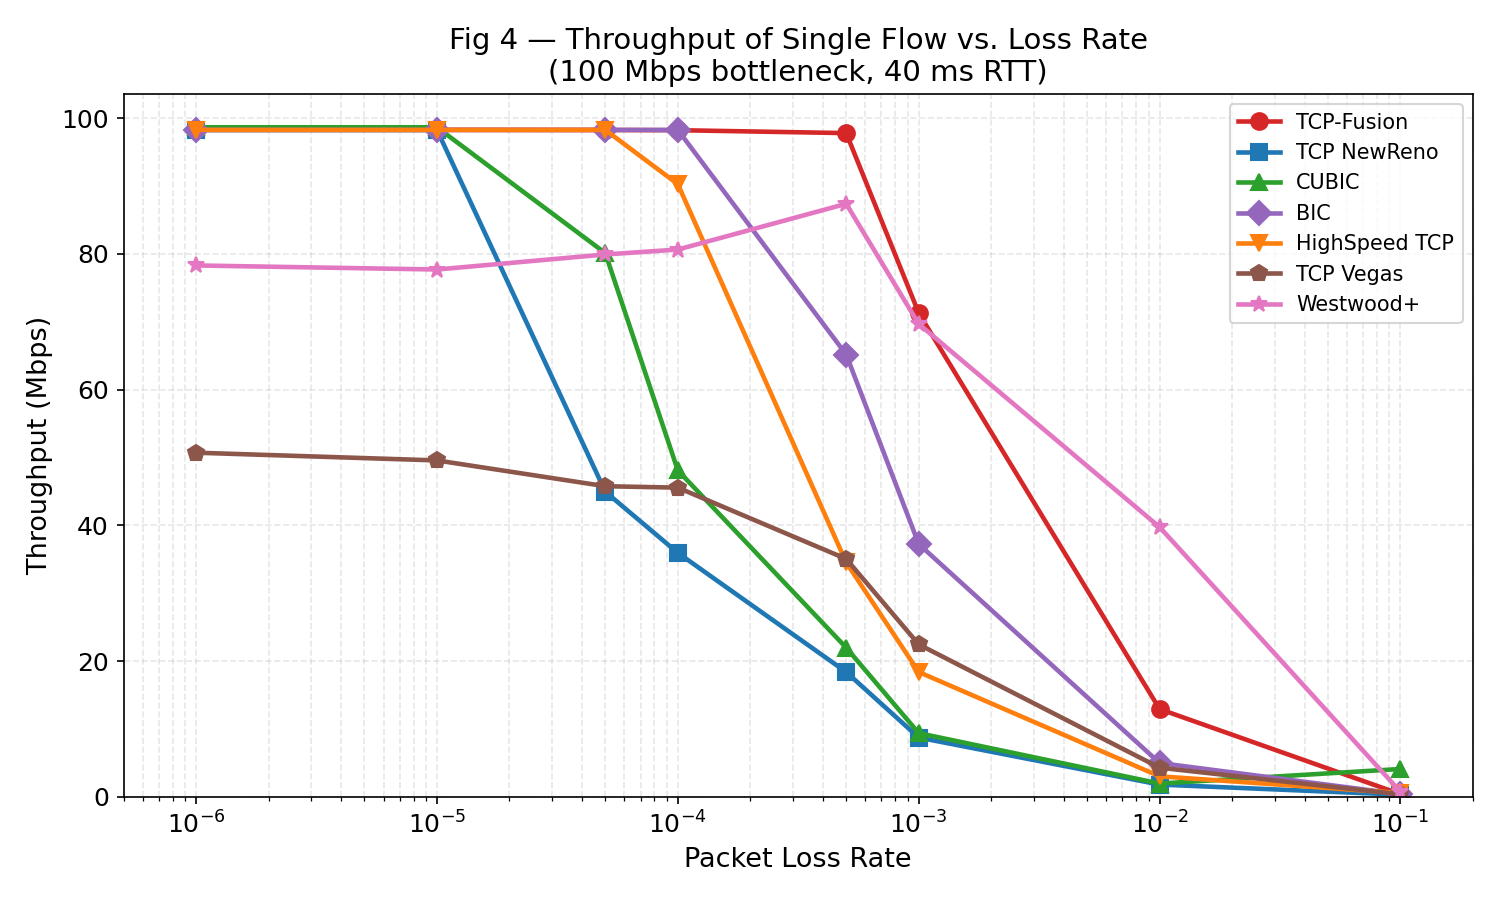
\includegraphics[width=0.82\textwidth]{figures/fig4_single_flow_throughput.png}
    \caption{\textbf{Single-Flow Throughput vs.\ Packet Loss Rate.} This figure compares the throughput resilience of TCP-Fusion against other TCP variants as the network packet loss rate is varied. TCP-Fusion maintains noticeably higher throughput at low-to-moderate loss rates compared to classic Reno. This improvement stems from the Vegas-like delay signal, which allows TCP-Fusion to react to growing queue pressure \textit{before} actual packet loss occurs, thereby avoiding unnecessary congestion window reductions.}
    \label{fig:fig4}
\end{figure}

\begin{figure}[htbp]
    \centering
    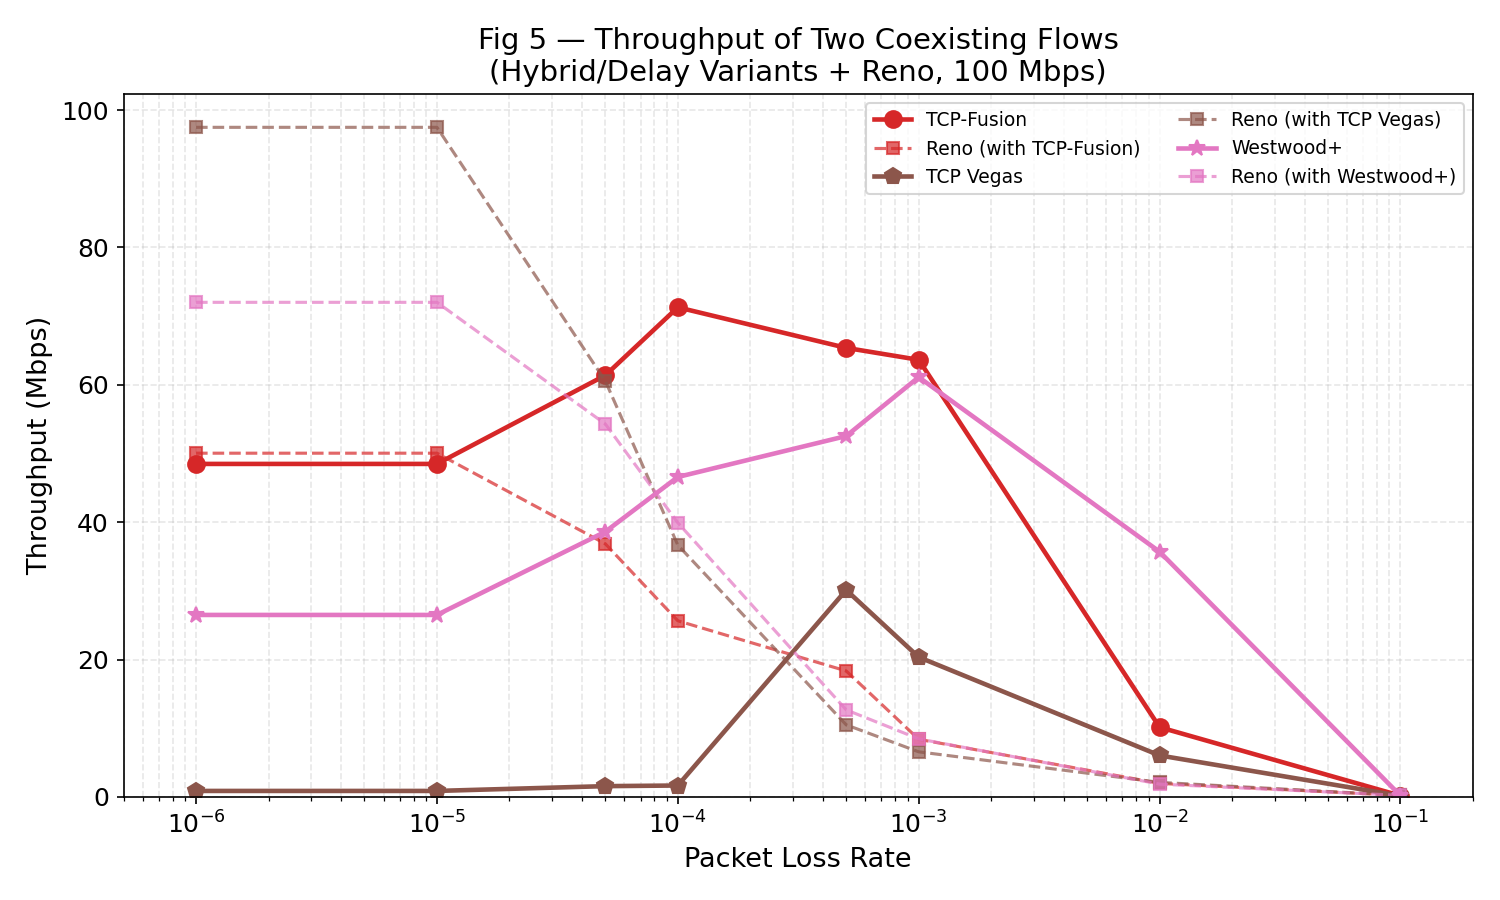
\includegraphics[width=0.82\textwidth]{figures/fig5_two_flows_hybrid.png}
    \caption{\textbf{Two-Flow Coexistence: TCP-Fusion vs.\ TCP Reno (Hybrid).} This figure evaluates the coexistence behavior when a TCP-Fusion flow competes simultaneously with a TCP Reno flow over the same bottleneck link. The key question is whether TCP-Fusion's improved throughput is a result of genuine efficiency or aggressive behavior that unfairly starves the Reno flow. A well-designed protocol should claim higher throughput without disproportionately reducing the competing flow's bandwidth share.}
    \label{fig:fig5}
\end{figure}

\begin{figure}[htbp]
    \centering
    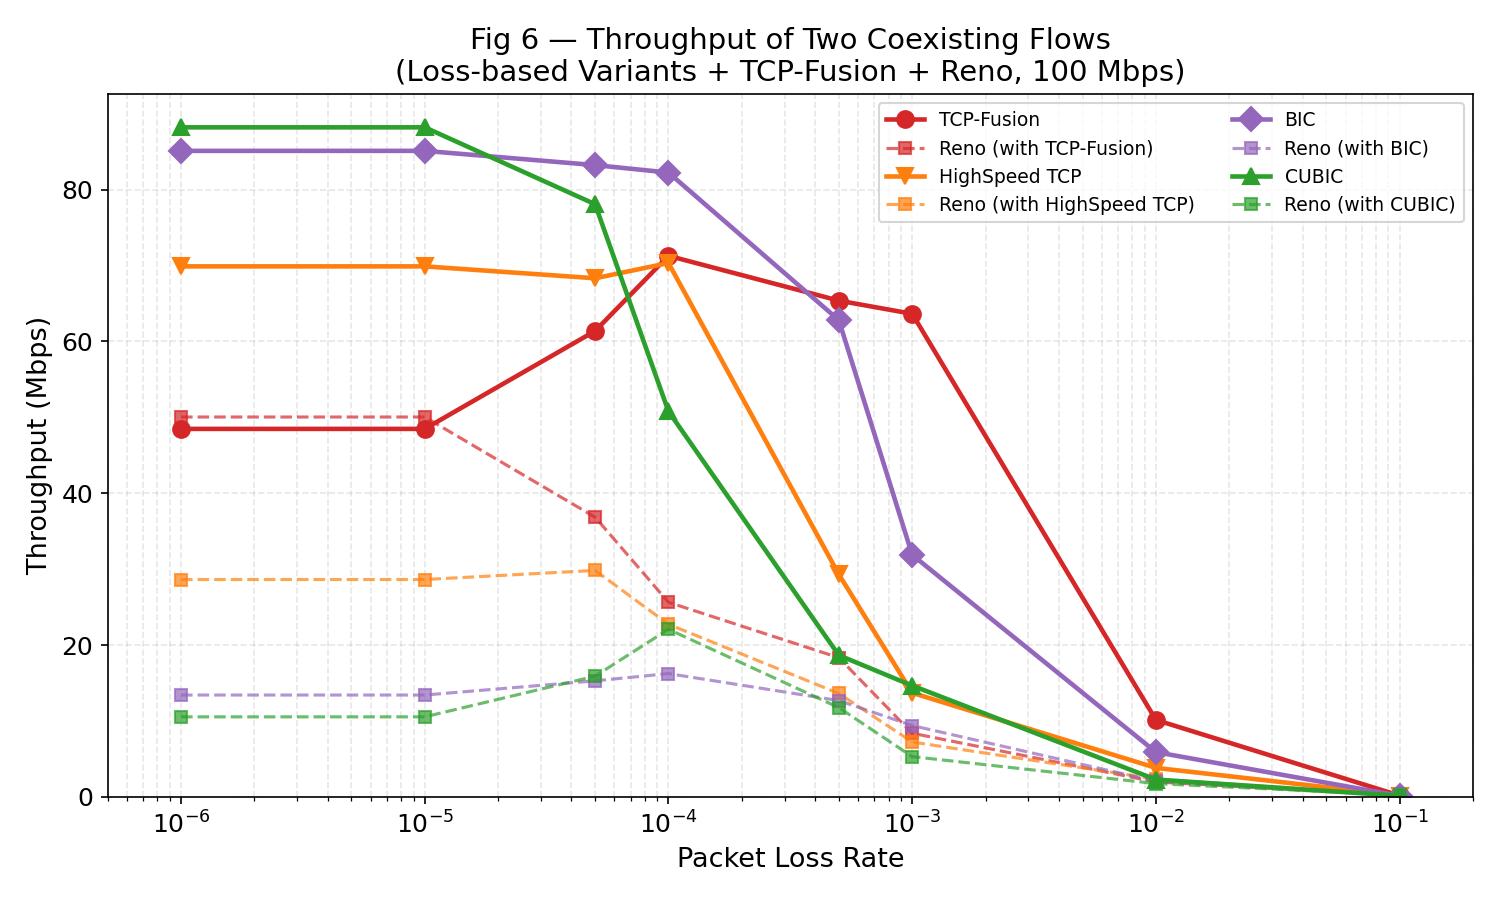
\includegraphics[width=0.82\textwidth]{figures/fig6_two_flows_lossbased.png}
    \caption{\textbf{Two-Flow Coexistence: Loss-Based Comparison with Fusion+Reno Curve.} An updated coexistence plot including a direct TCP-Fusion vs.\ TCP Reno comparison curve under loss-based conditions. This figure complements Figure~\ref{fig:fig5} by isolating the loss-driven dimension of coexistence, making it easier to observe how each protocol's window reduction behavior affects the bandwidth share of a competing flow under varying loss conditions.}
    \label{fig:fig6}
\end{figure}

\begin{figure}[htbp]
    \centering
    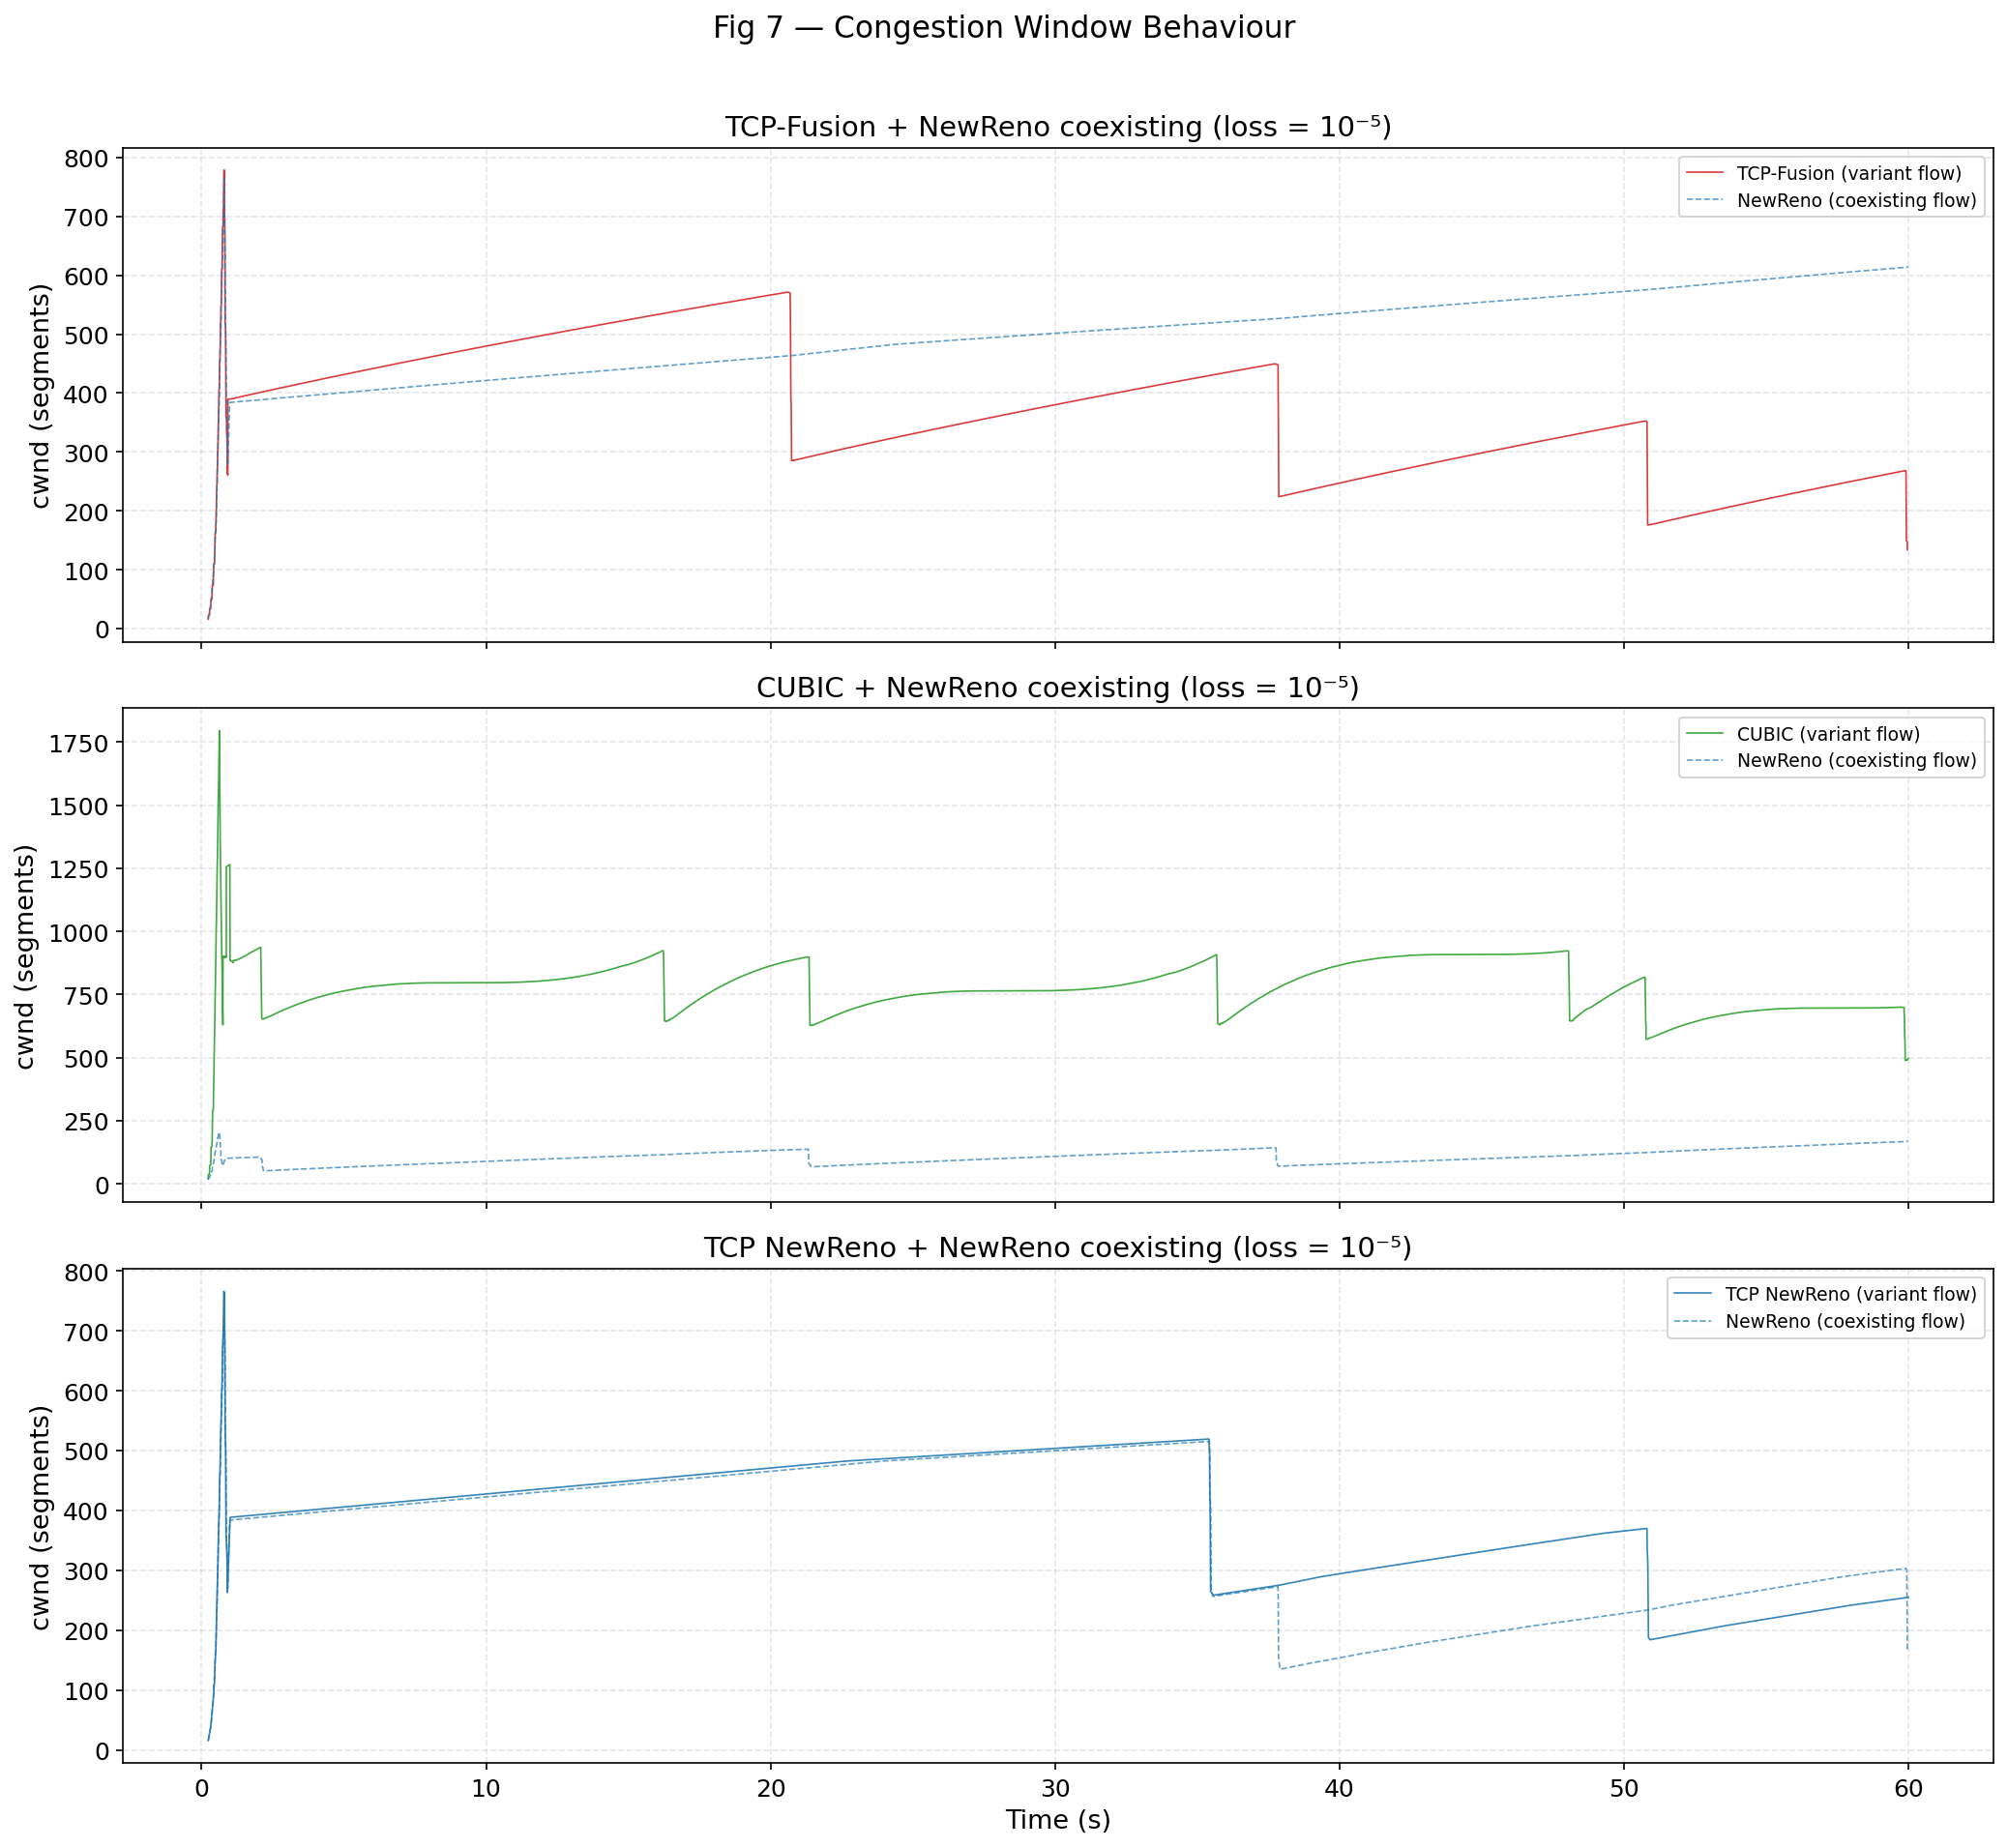
\includegraphics[width=0.82\textwidth]{figures/fig7_cwnd_behaviour.png}
    \caption{\textbf{Congestion Window (cwnd) Time-Domain Behaviour.} This figure shows the evolution of the congestion window size over simulation time for TCP-Fusion compared to other variants. Key aspects visible include oscillation smoothness (a smoother cwnd trace indicates more stable throughput), reaction speed to congestion events, and recovery time after a loss event. The cwnd trace provides the mechanistic explanation for why TCP-Fusion achieves its observed throughput outcomes --- the delay-awareness of Fusion prevents the sharp sawtooth pattern typical of Reno.}
    \label{fig:fig7}
\end{figure}

\begin{figure}[htbp]
    \centering
    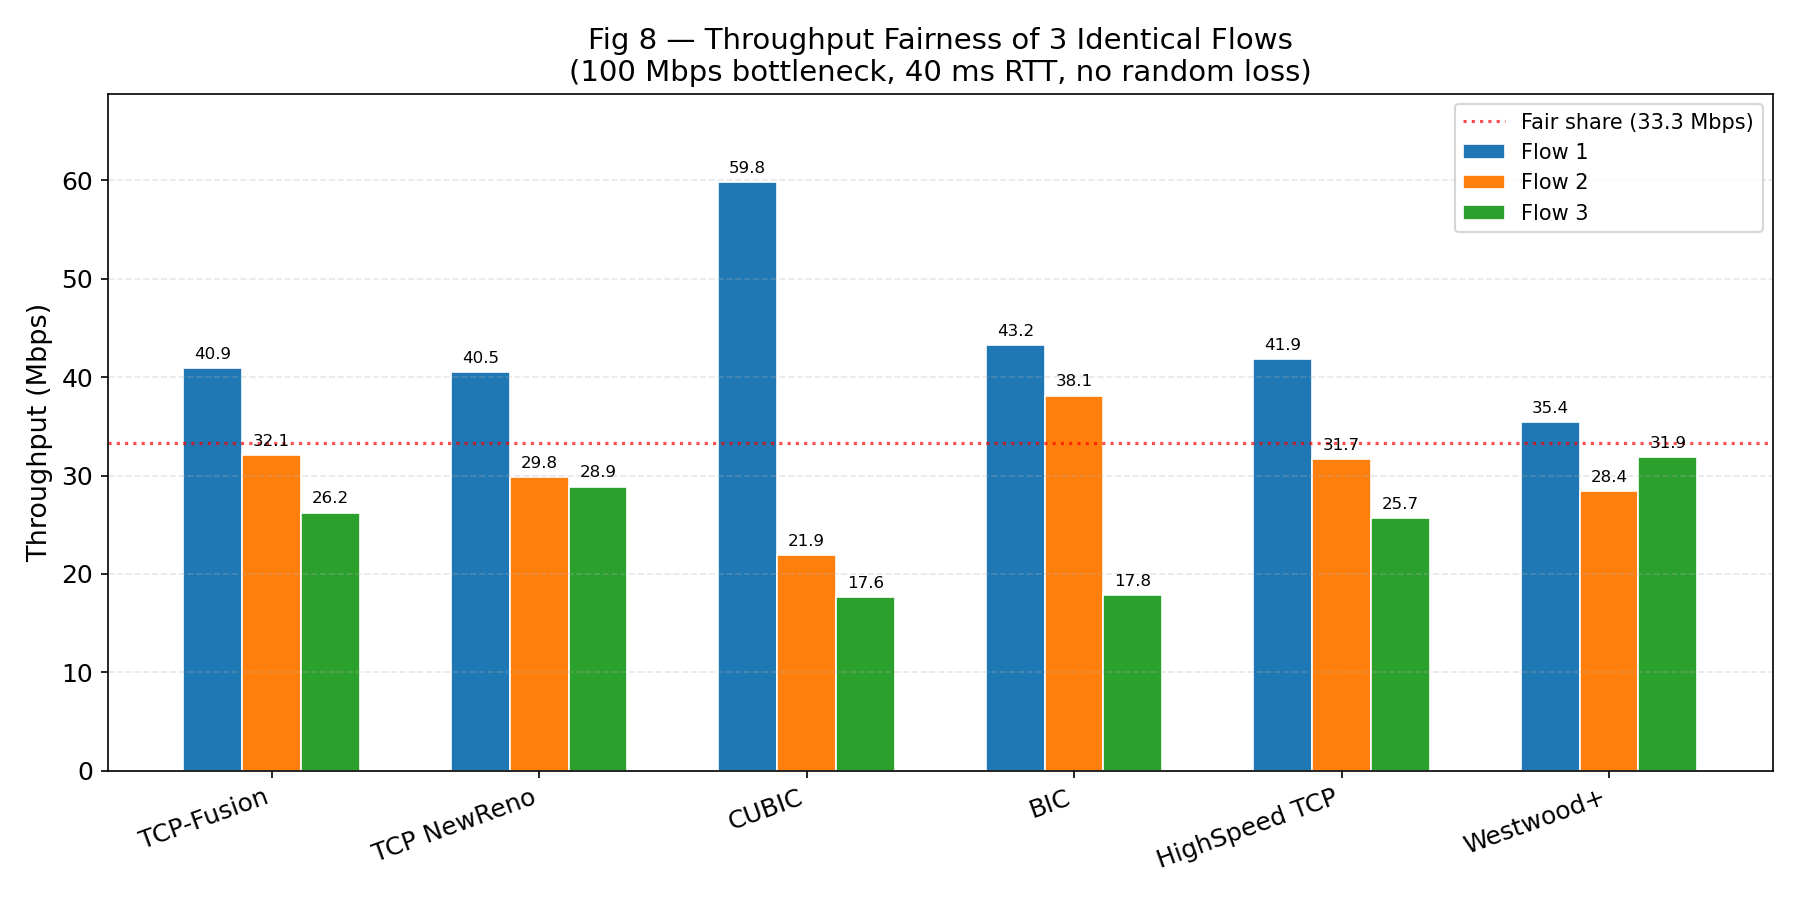
\includegraphics[width=0.82\textwidth]{figures/fig8_three_flows_fairness.png}
    \caption{\textbf{Three Identical TCP-Fusion Flows --- Intra-Protocol Fairness.} This figure evaluates intra-protocol fairness when three simultaneous TCP-Fusion flows compete over the same bottleneck. A fair protocol should distribute bandwidth roughly equally among all competing flows. Results demonstrate that TCP-Fusion achieves good intra-protocol fairness, outperforming strongly aggressive protocols such as CUBIC in this setup, where CUBIC's cubic window growth function can cause one flow to dominate the others over time.}
    \label{fig:fig8}
\end{figure}

\FloatBarrier

\subsection{Extra graphs inspired by the CUBIC paper}

To fill that gap, we added CUBIC-style experiments and then generated the same style for TCP-Fusion. These extra figures helped us see:
\begin{itemize}
    \item how quickly one protocol starts dominating another over time,
    \item how RTT changes friendliness,
    \item and how bandwidth changes the share taken by each protocol.
\end{itemize}

In short, the first set told us \textit{what} performance we got; the CUBIC-style set explained \textit{why} and \textit{under which conditions} fairness changes.

\begin{figure}[htbp]
    \centering
    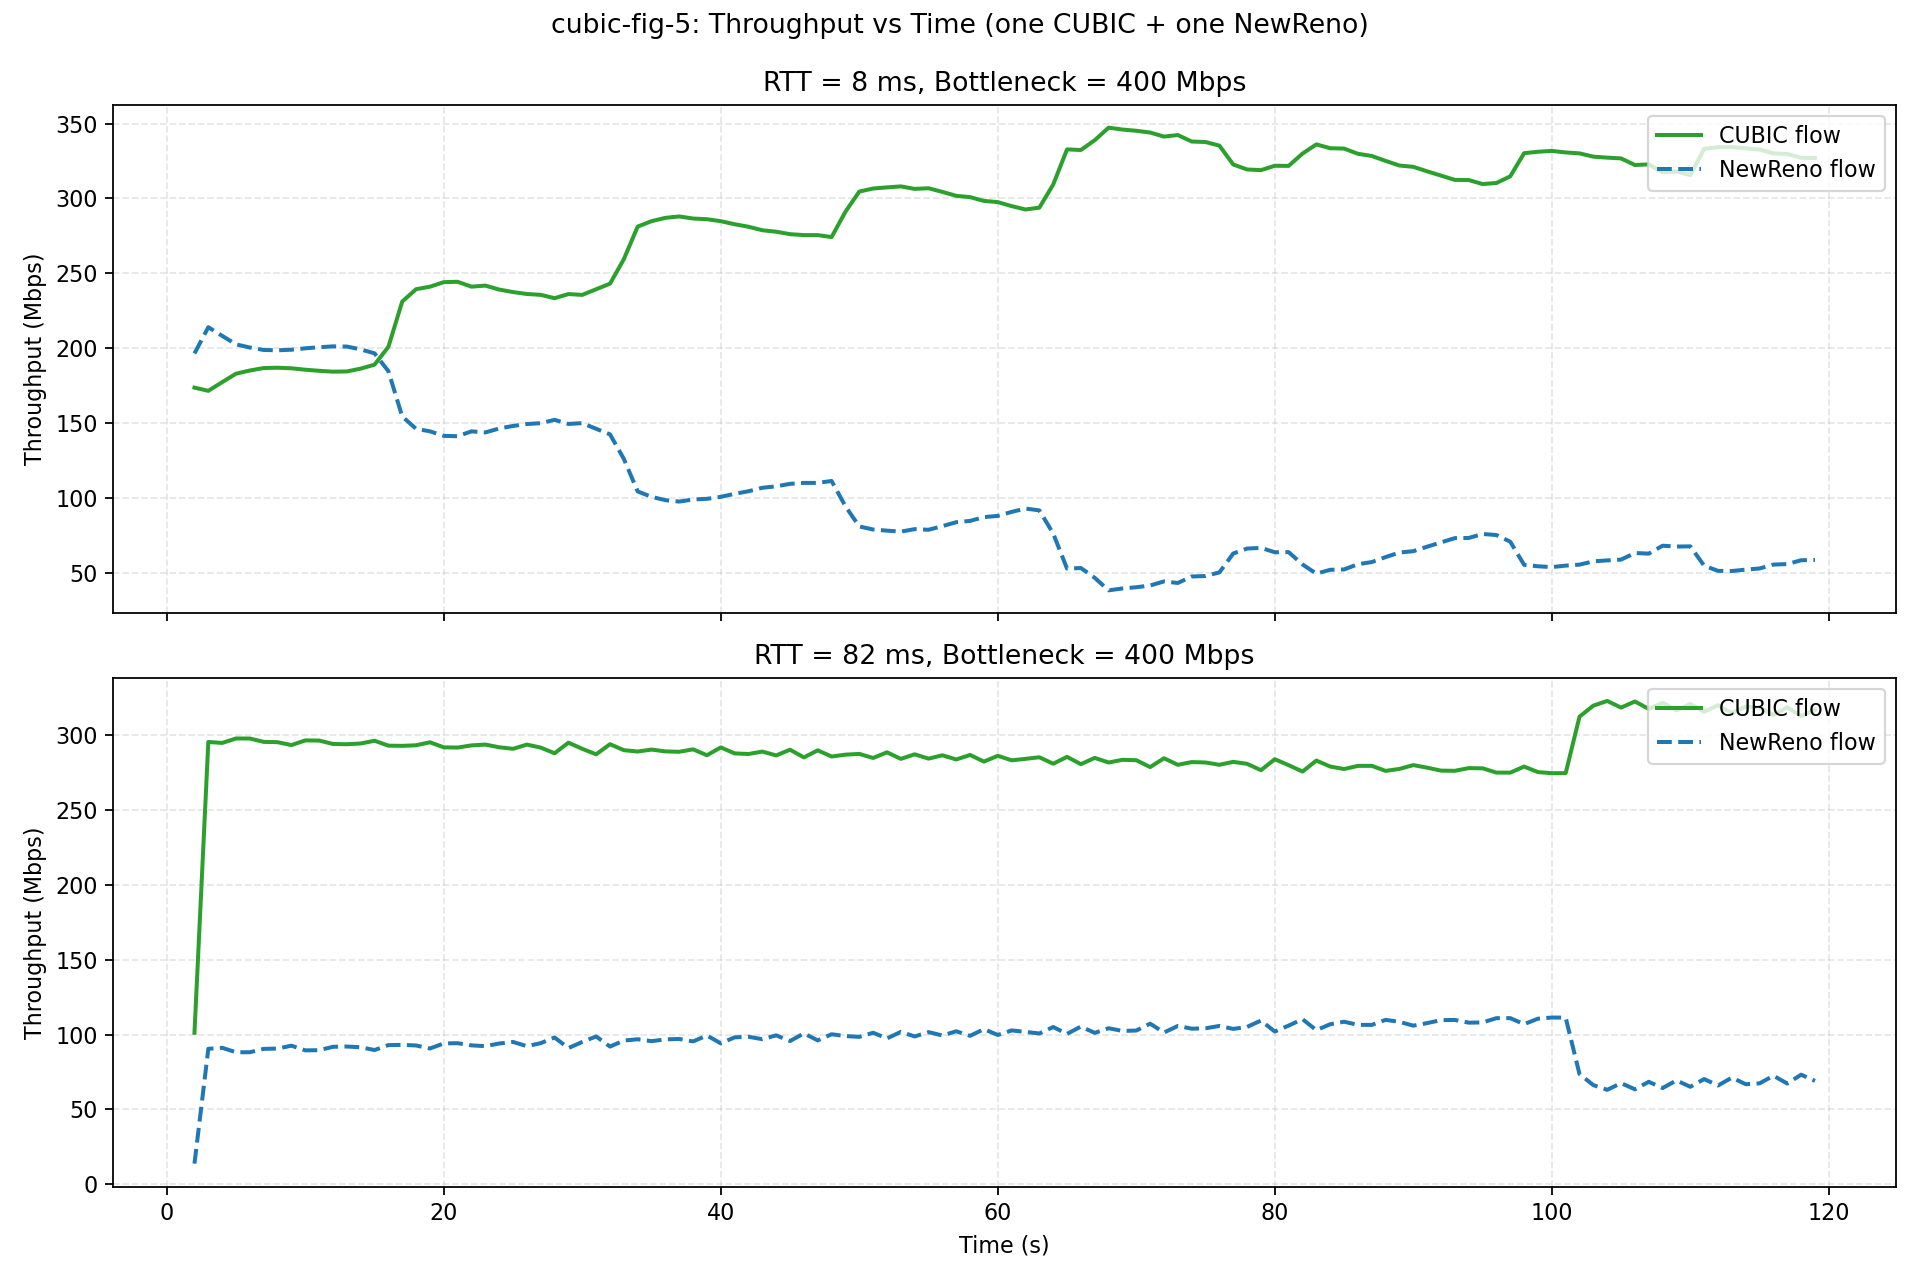
\includegraphics[width=0.82\textwidth]{figures/cubic-fig-5.png}
    \caption{\textbf{CUBIC vs.\ NewReno: Throughput vs.\ Time at RTT = 8ms and 82ms.} Reproduced from the CUBIC paper experimental setup, this figure shows the time-evolution of throughput when CUBIC competes with NewReno at two different RTT values. At low RTT (8ms), both protocols behave similarly since BDP is small. At high RTT (82ms), CUBIC's cubic window growth function allows it to ramp up significantly faster than NewReno, demonstrating CUBIC's RTT-independence advantage in high-BDP conditions where NewReno's linear growth is insufficient.}
    \label{fig:cubic5}
\end{figure}

\FloatBarrier

\begin{figure}[htbp]
    \centering
    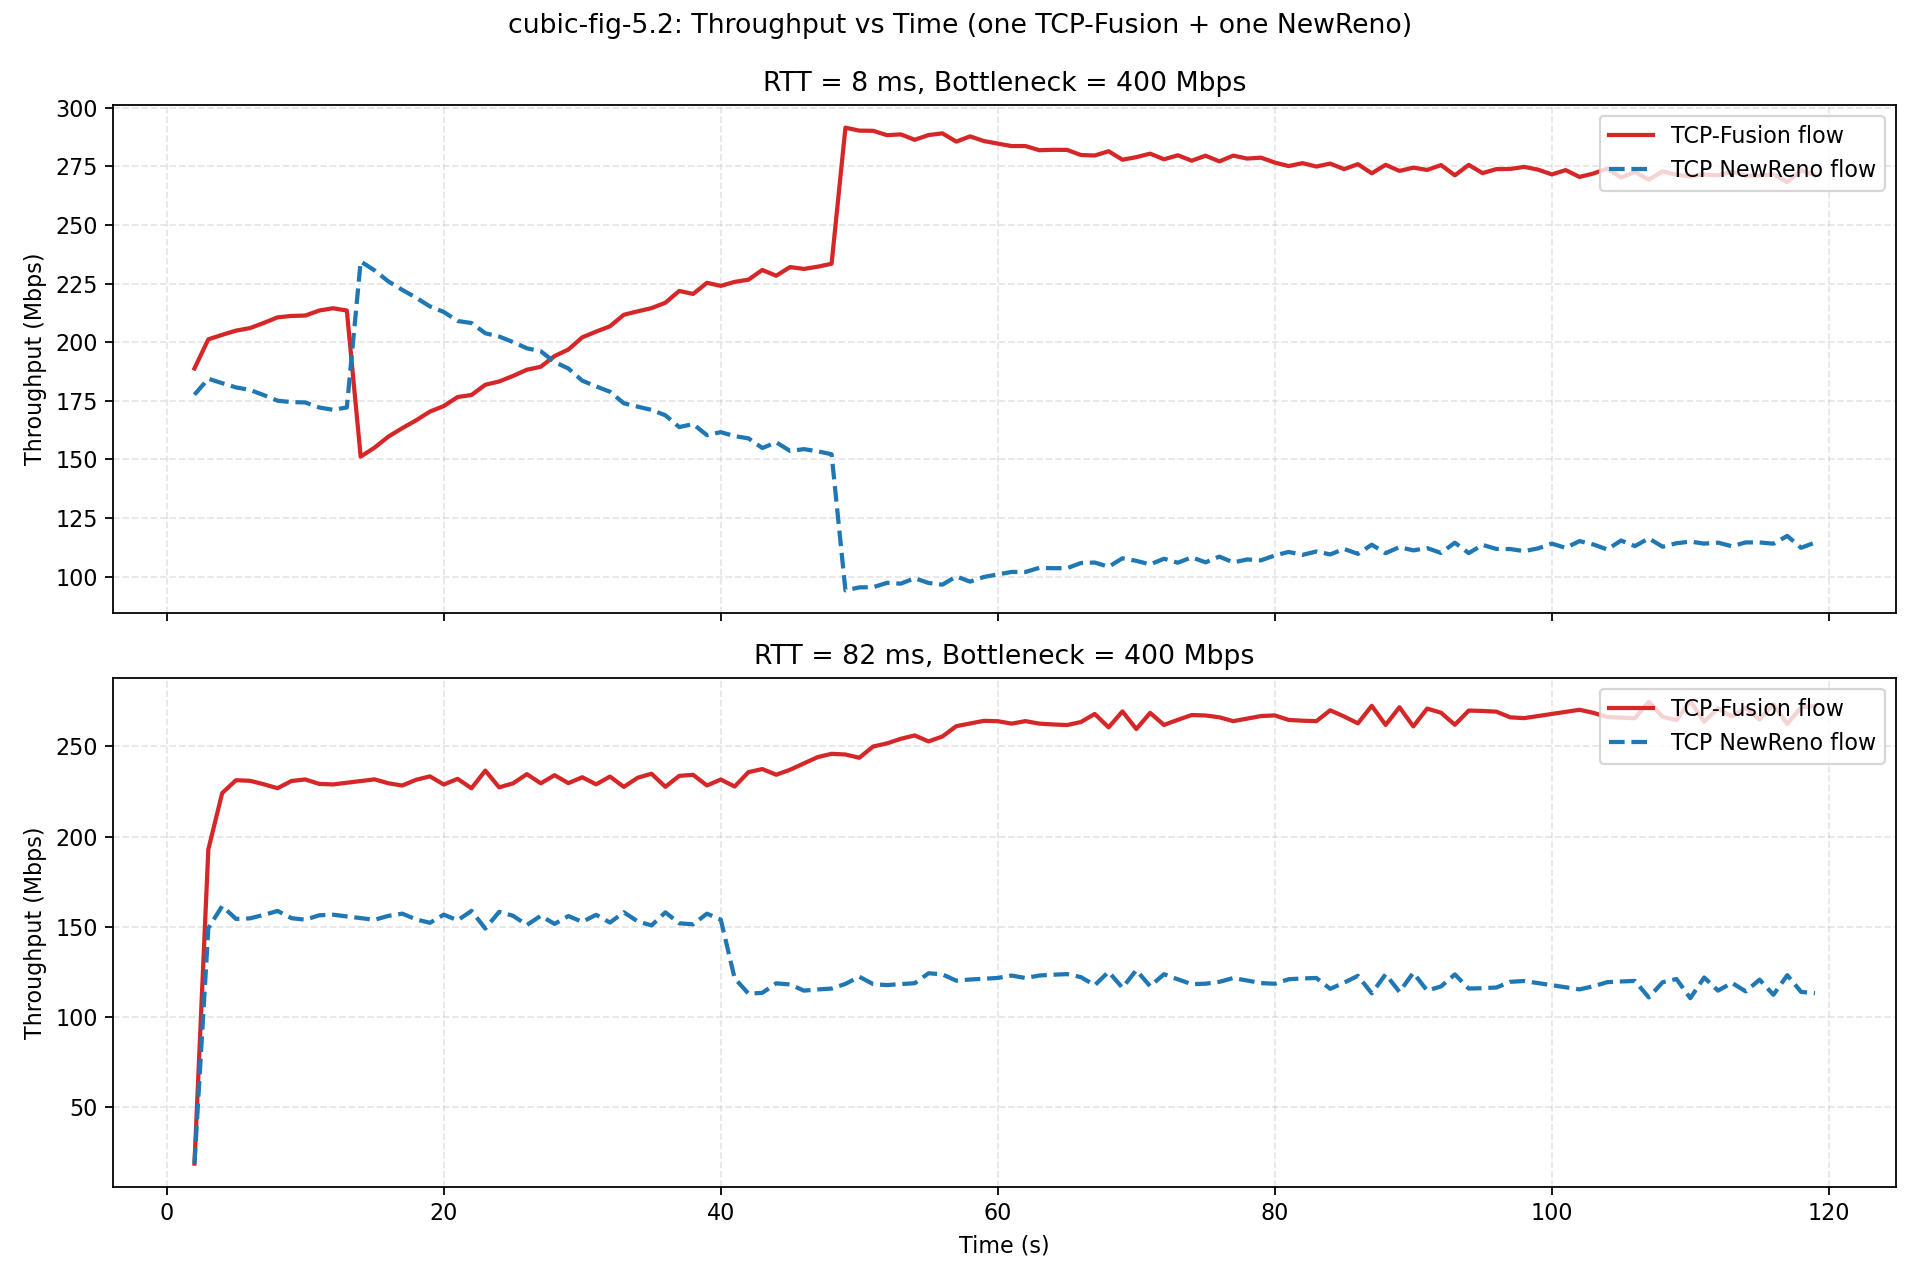
\includegraphics[width=0.82\textwidth]{figures/cubic-fig-5.2.png}
    \caption{\textbf{TCP-Fusion vs.\ NewReno: Throughput vs.\ Time at RTT = 8ms and 82ms.} The TCP-Fusion equivalent of Figure~\ref{fig:cubic5}, directly comparing TCP-Fusion against NewReno under identical RTT conditions. This figure reveals whether TCP-Fusion exhibits time-domain dominance similar to CUBIC or a more balanced coexistence with NewReno. Unlike CUBIC, TCP-Fusion's delay-awareness is expected to prevent runaway window growth, resulting in a more gradual and stable throughput increase that avoids unfairly starving the competing NewReno flow.}
    \label{fig:cubic52}
\end{figure}

\begin{figure}[htbp]
    \centering
    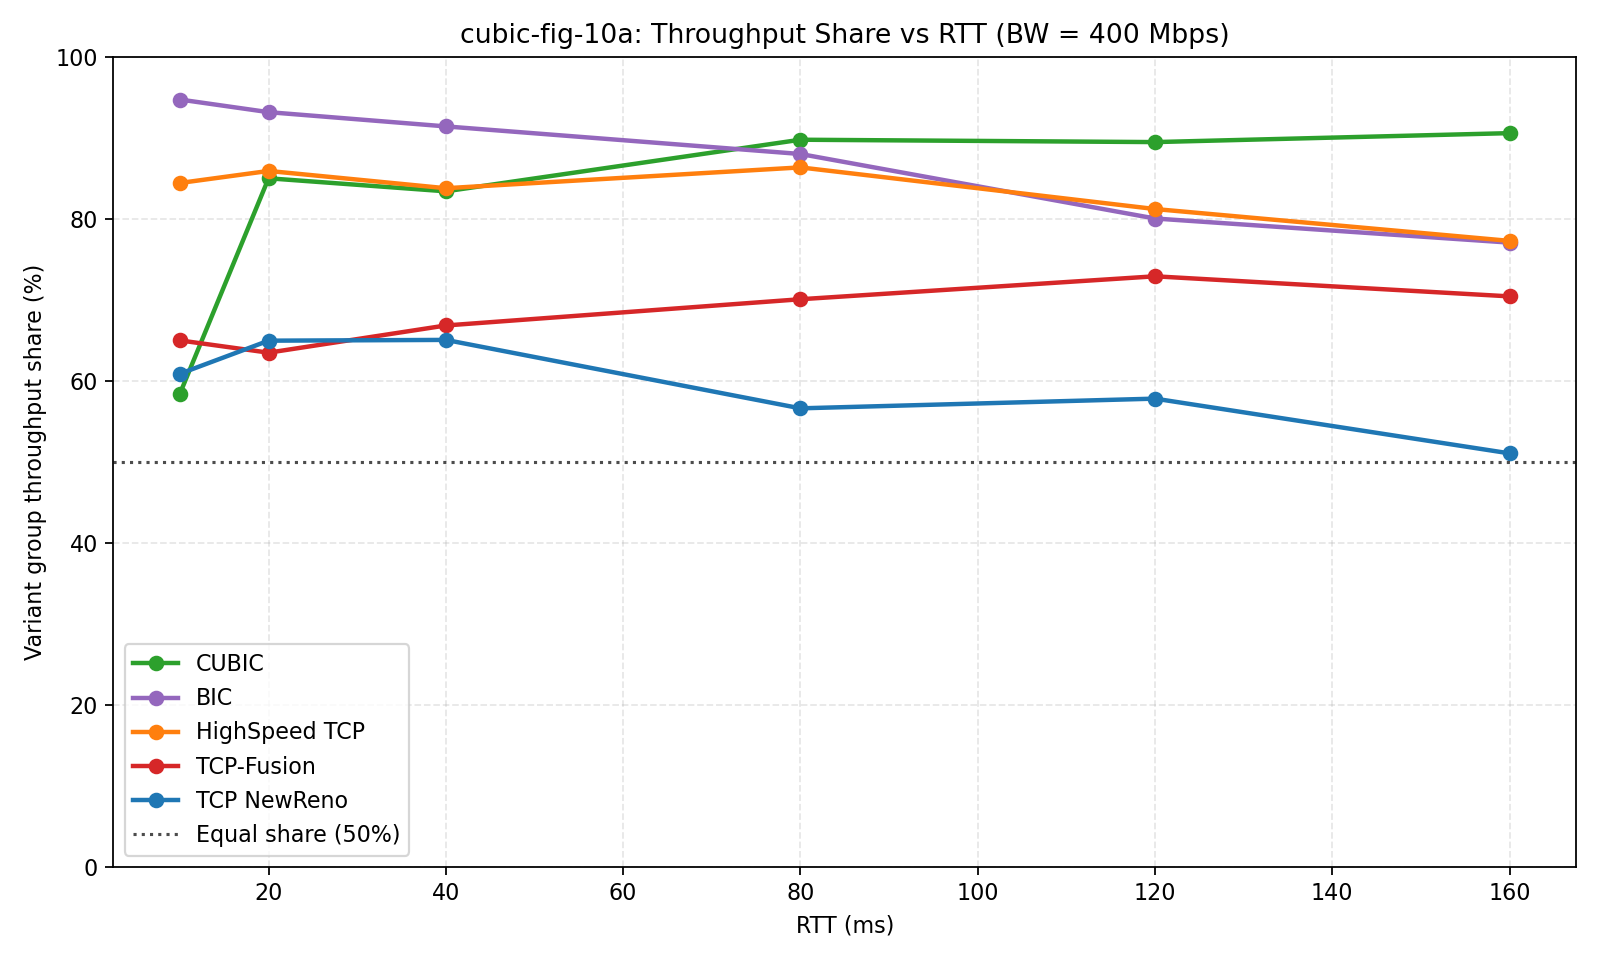
\includegraphics[width=0.82\textwidth]{figures/cubic-fig-10a.png}
    \caption{\textbf{Throughput Share vs.\ RTT (Bandwidth Fixed).} This figure plots the throughput \textit{share} --- the fraction of total bottleneck bandwidth claimed by each competing protocol --- as RTT is varied while keeping bandwidth fixed. Each data point is a run-average share over the full simulation duration, not an instantaneous measurement. A share consistently above 50\% indicates aggressiveness at the expense of the competing flow. This figure exposes fairness properties that raw throughput numbers alone cannot reveal, especially under high RTT where window growth rates diverge significantly between protocols.}
    \label{fig:cubic10a}
\end{figure}

\begin{figure}[htbp]
    \centering
    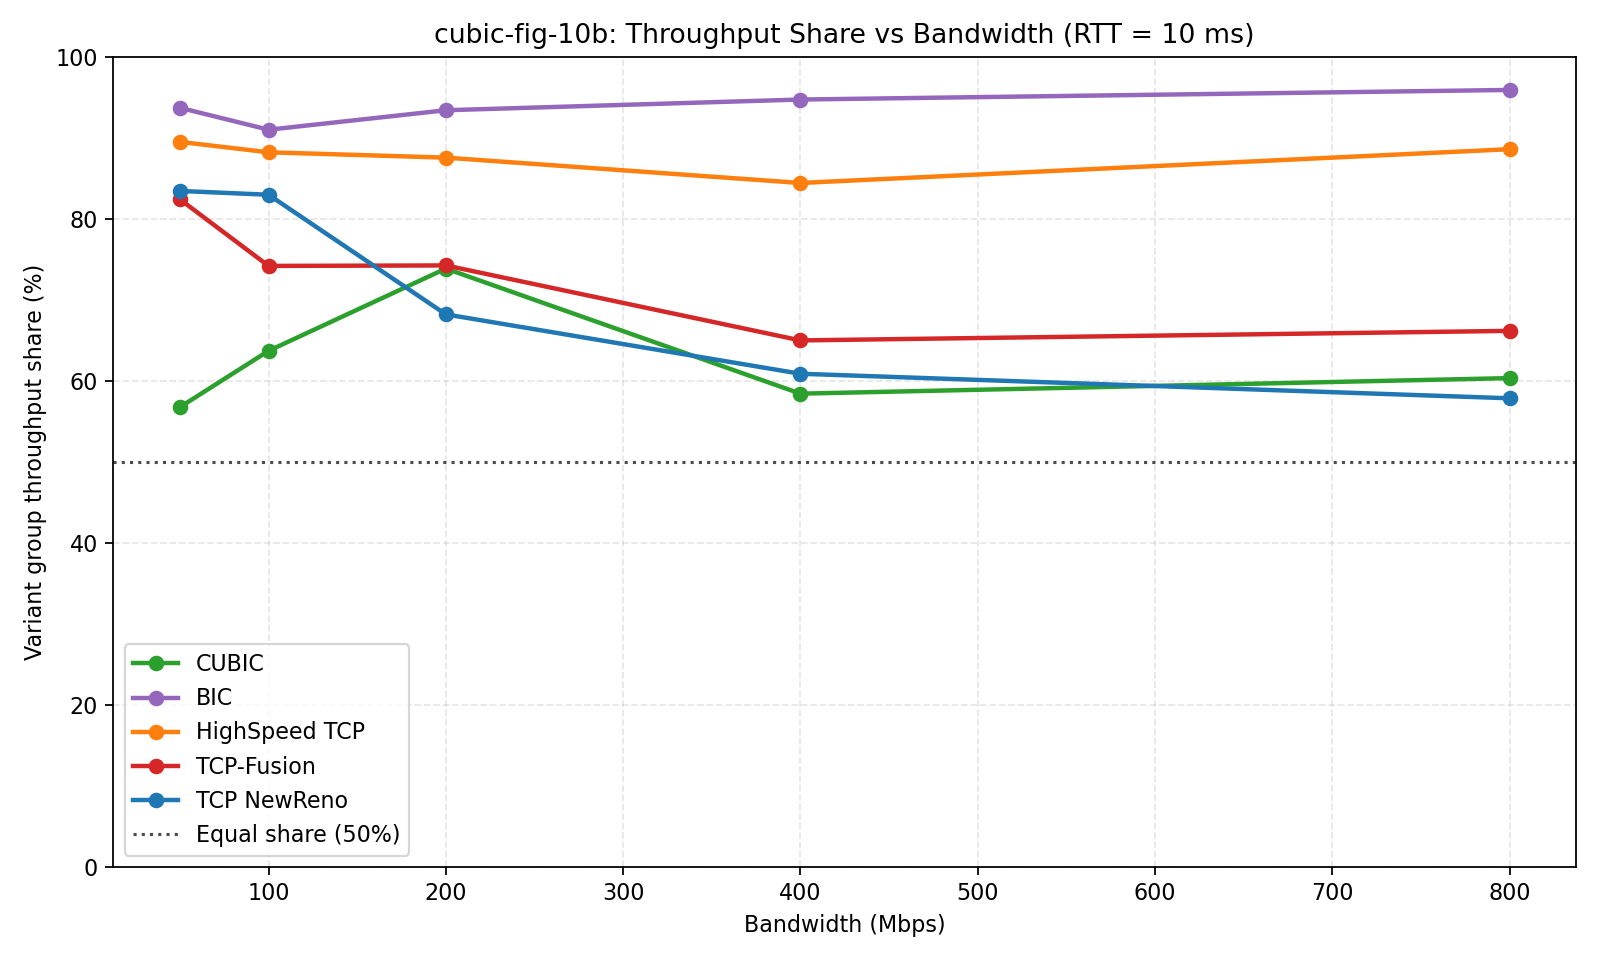
\includegraphics[width=0.82\textwidth]{figures/cubic-fig-10b.png}
    \caption{\textbf{Throughput Share vs.\ Bandwidth (RTT = 10ms).} At low RTT (10ms), this figure shows how throughput share between competing protocols changes as bottleneck bandwidth increases. At low RTT the BDP is small and most TCP variants behave similarly, so throughput shares are expected to remain relatively balanced across bandwidth values. Any deviations indicate protocol-specific behaviors triggered by higher capacity availability even under low-latency conditions.}
    \label{fig:cubic10b}
\end{figure}

\begin{figure}[htbp]
    \centering
    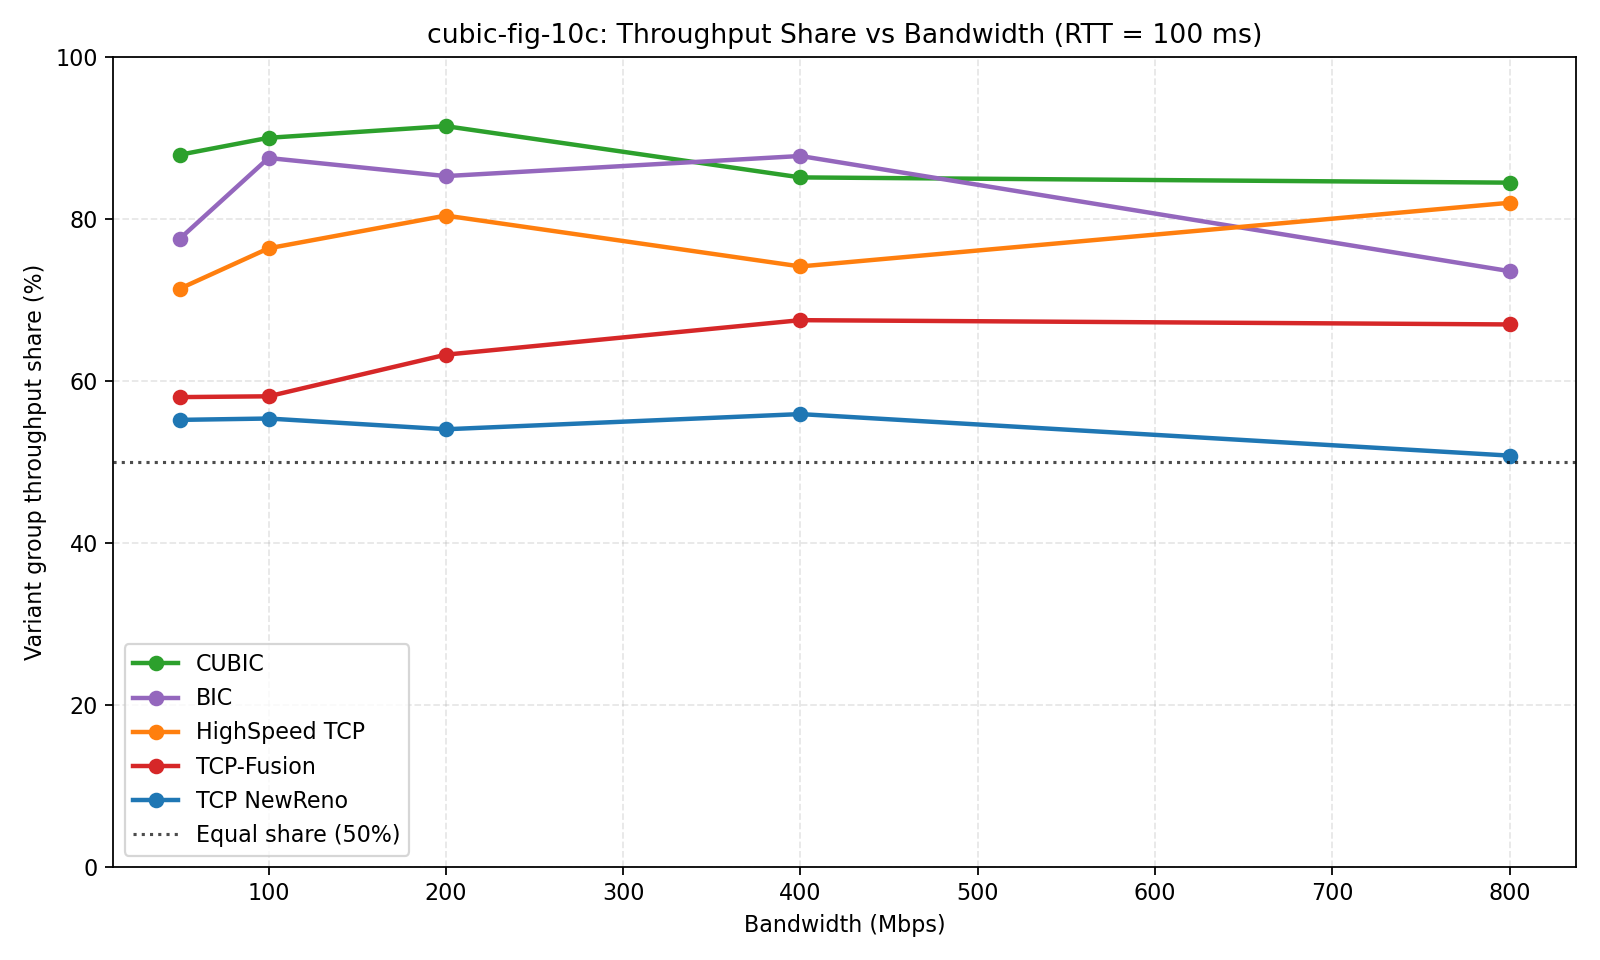
\includegraphics[width=0.82\textwidth]{figures/cubic-fig-10c.png}
    \caption{\textbf{Throughput Share vs.\ Bandwidth (RTT = 100ms).} At high RTT (100ms), the BDP is large and differences between TCP variants become pronounced. This figure shows how throughput share evolves as bandwidth increases under high-latency conditions. Protocols designed for high-BDP environments (such as CUBIC and TCP-Fusion) are expected to claim a larger share compared to NewReno, which suffers from slow linear window growth under high RTT. The comparison between this figure and Figure~\ref{fig:cubic10b} illustrates the RTT-sensitivity of each protocol's aggressiveness.}
    \label{fig:cubic10c}
\end{figure}

% -----------------------------------------------
\section{Assigned Mobile Wireless Experiments}

\subsection{Assignment Specification}

The assigned network types are:

\begin{itemize}
    \item \textbf{Wireless 802.11 (mobile)}
    \item \textbf{Wireless 802.15.4 (mobile)}
\end{itemize}

\subsection{Network Topologies}

\subsubsection{IEEE 802.11 Mobile (Ad-hoc WiFi)}
\begin{itemize}
    \item Standard: 802.11g, Ad-hoc mode (no fixed Access Point)
    \item Routing Protocol: AODV (Ad-hoc On-Demand Distance Vector)
    \item Mobility Model: Random Waypoint
    \item Simulation Area: Square flat grid
    \item Energy Model: NS-3 WiFi Radio Energy Model
\end{itemize}

\subsubsection{IEEE 802.15.4 Mobile (LR-WPAN / Zigbee)}
\begin{itemize}
    \item Stack: LR-WPAN + 6LoWPAN + IPv6
    \item Mobility Model: Random Waypoint
    \item Energy Model: Analytical estimate (Tx/Rx/Idle power terms)
    \item Max Frame Size: 127 bytes (causes TCP segment fragmentation via 6LoWPAN)
\end{itemize}

\textbf{Note:} Absolute energy values across WiFi and LR-WPAN are \textit{not} directly comparable due to different energy modeling approaches. This is explicitly documented to avoid unfair cross-technology energy claims.

\subsection{Parameters Varied}

Since both assigned networks involve \textbf{mobile} nodes, the coverage area is fixed and node speed is varied instead. The parameters varied are:

\begin{table}[htbp]
\centering
\caption{Simulation Parameters}
\begin{tabular}{@{}lll@{}}
\toprule
\textbf{Parameter} & \textbf{Values} & \textbf{Baseline} \\
\midrule
Number of Nodes & 20, 40, 60, 80, 100 & 60 \\
Number of Flows & 10, 20, 30, 40, 50 & 30 \\
Packets per Second & 100, 200, 300, 400, 500 & 300 \\
Node Speed (m/s) & 5, 10, 15, 20, 25 & 15 \\
\bottomrule
\end{tabular}
\end{table}

When varying one parameter, all others are held at their baseline value.

\subsection{Metrics Measured}

The following metrics are collected and plotted for each parameter variation:

\begin{enumerate}
    \item \textbf{Network Throughput} (Mbps)
    \item \textbf{End-to-End Delay} (ms)
    \item \textbf{Packet Delivery Ratio (PDR)} = $\frac{\text{total packets received}}{\text{total packets sent}}$
    \item \textbf{Packet Drop Ratio} = $\frac{\text{total packets dropped}}{\text{total packets sent}}$
    \item \textbf{Energy Consumption} (Joules) --- applicable for all wireless nodes
\end{enumerate}

\subsection{Implementation Files}

The assigned experiments are located under \texttt{scratch/assigned\_experiments/}:

\begin{lstlisting}
tcp-fusion-wifi-mobile.cc       # 802.11 mobile simulation script
tcp-fusion-lrwpan-mobile.cc     # 802.15.4 mobile simulation script
run_mobile_experiments.py       # Automation script for all runs
plot_mobile_metrics.py          # Plotting pipeline
config_mobile.json              # Experiment configuration
README.md                       # Instructions
REPORT_TEMPLATE.md              # Report template
results/mobile_raw_results.csv  # Generated raw data
results/plots/                  # Generated plots
\end{lstlisting}

% -----------------------------------------------
\section{Results and Observations}

\subsection{Baseline Comparison}

At baseline parameters (nNodes = 60, nFlows = 30, pktPerSec = 300, speed = 15 m/s):

\begin{table}[htbp]
\centering
\caption{Baseline Performance: WiFi vs.\ LR-WPAN (TCP-Fusion)}
\begin{tabular}{@{}lccccc@{}}
\toprule
\textbf{Network} & \textbf{Throughput} & \textbf{Delay} & \textbf{PDR} & \textbf{Drop Ratio} & \textbf{Energy} \\
\midrule
WiFi 802.11 (mobile) & 2.794 Mbps & 27.50 ms & 0.8928 & 0.1072 & 2995.59 J \\
LR-WPAN 802.15.4 (mobile) & 0.0905 Mbps & 291.23 ms & 0.7011 & 0.2989 & 11.36 J \\
\bottomrule
\end{tabular}
\end{table}

WiFi delivers substantially higher throughput and much lower delay compared to LR-WPAN. LR-WPAN's energy consumption is orders of magnitude lower, consistent with its low-power sensor network design.

\subsection{Parameter Variation Trends}

\subsubsection{A) Varying Number of Nodes}
\begin{itemize}
    \item \textbf{WiFi:} Throughput falls significantly as nodes increase due to channel contention and route instability. Delay and drop ratio increase.
    \item \textbf{LR-WPAN:} Throughput remains around $\sim$0.09 Mbps regardless of node count; delay is persistently high, and reliability is moderate-to-low.
\end{itemize}

\subsubsection{B) Varying Number of Flows}
\begin{itemize}
    \item \textbf{WiFi:} Total throughput increases with more flows up to channel saturation, but delay and drops also rise.
    \item \textbf{LR-WPAN:} Throughput saturates early; additional flows primarily increase delay and drop ratio, significantly reducing PDR.
\end{itemize}

\subsubsection{C) Varying Packet Rate}
\begin{itemize}
    \item \textbf{WiFi:} Throughput grows with offered load and PDR remains comparatively stable.
    \item \textbf{LR-WPAN:} Only marginal throughput gains; high delay persists, indicating a bottlenecked MAC/PHY layer incapable of handling high offered loads.
\end{itemize}

\subsubsection{D) Varying Node Speed}
\begin{itemize}
    \item \textbf{WiFi:} Higher speed degrades throughput and PDR while increasing drops, due to more frequent topology changes and AODV route breaks.
    \item \textbf{LR-WPAN:} Speed impact is weaker than load impact; overall throughput stays in a narrow low band regardless of speed.
\end{itemize}

\subsection{Assigned Experiment Plots }

\subsubsection{Throughput}
\MobilePairPlot{wifi-mobile_throughput_vs_nNodes.png}{lrwpan-mobile_throughput_vs_nNodes.png}{Throughput vs Number of Nodes}{fig:assgn_thr_nodes}
\MobilePairPlot{wifi-mobile_throughput_vs_nFlows.png}{lrwpan-mobile_throughput_vs_nFlows.png}{Throughput vs Number of Flows}{fig:assgn_thr_flows}
\MobilePairPlot{wifi-mobile_throughput_vs_pktPerSec.png}{lrwpan-mobile_throughput_vs_pktPerSec.png}{Throughput vs Packet Rate}{fig:assgn_thr_pkt}
\MobilePairPlot{wifi-mobile_throughput_vs_speed.png}{lrwpan-mobile_throughput_vs_speed.png}{Throughput vs Node Speed}{fig:assgn_thr_speed}
\FloatBarrier

\subsubsection{End-to-End Delay}
\MobilePairPlot{wifi-mobile_delay_vs_nNodes.png}{lrwpan-mobile_delay_vs_nNodes.png}{End-to-End Delay vs Number of Nodes}{fig:assgn_delay_nodes}
\MobilePairPlot{wifi-mobile_delay_vs_nFlows.png}{lrwpan-mobile_delay_vs_nFlows.png}{End-to-End Delay vs Number of Flows}{fig:assgn_delay_flows}
\MobilePairPlot{wifi-mobile_delay_vs_pktPerSec.png}{lrwpan-mobile_delay_vs_pktPerSec.png}{End-to-End Delay vs Packet Rate}{fig:assgn_delay_pkt}
\MobilePairPlot{wifi-mobile_delay_vs_speed.png}{lrwpan-mobile_delay_vs_speed.png}{End-to-End Delay vs Node Speed}{fig:assgn_delay_speed}
\FloatBarrier

\subsubsection{Packet Delivery Ratio (PDR)}
\MobilePairPlot{wifi-mobile_pdr_vs_nNodes.png}{lrwpan-mobile_pdr_vs_nNodes.png}{PDR vs Number of Nodes}{fig:assgn_pdr_nodes}
\MobilePairPlot{wifi-mobile_pdr_vs_nFlows.png}{lrwpan-mobile_pdr_vs_nFlows.png}{PDR vs Number of Flows}{fig:assgn_pdr_flows}
\MobilePairPlot{wifi-mobile_pdr_vs_pktPerSec.png}{lrwpan-mobile_pdr_vs_pktPerSec.png}{PDR vs Packet Rate}{fig:assgn_pdr_pkt}
\MobilePairPlot{wifi-mobile_pdr_vs_speed.png}{lrwpan-mobile_pdr_vs_speed.png}{PDR vs Node Speed}{fig:assgn_pdr_speed}
\FloatBarrier

\subsubsection{Packet Drop Ratio}
\MobilePairPlot{wifi-mobile_drop_vs_nNodes.png}{lrwpan-mobile_drop_vs_nNodes.png}{Drop Ratio vs Number of Nodes}{fig:assgn_drop_nodes}
\MobilePairPlot{wifi-mobile_drop_vs_nFlows.png}{lrwpan-mobile_drop_vs_nFlows.png}{Drop Ratio vs Number of Flows}{fig:assgn_drop_flows}
\MobilePairPlot{wifi-mobile_drop_vs_pktPerSec.png}{lrwpan-mobile_drop_vs_pktPerSec.png}{Drop Ratio vs Packet Rate}{fig:assgn_drop_pkt}
\MobilePairPlot{wifi-mobile_drop_vs_speed.png}{lrwpan-mobile_drop_vs_speed.png}{Drop Ratio vs Node Speed}{fig:assgn_drop_speed}
\FloatBarrier

\subsubsection{Energy Consumption}
\MobilePairPlot{wifi-mobile_energy_vs_nNodes.png}{lrwpan-mobile_energy_vs_nNodes.png}{Energy Consumption vs Number of Nodes}{fig:assgn_energy_nodes}
\MobilePairPlot{wifi-mobile_energy_vs_nFlows.png}{lrwpan-mobile_energy_vs_nFlows.png}{Energy Consumption vs Number of Flows}{fig:assgn_energy_flows}
\MobilePairPlot{wifi-mobile_energy_vs_pktPerSec.png}{lrwpan-mobile_energy_vs_pktPerSec.png}{Energy Consumption vs Packet Rate}{fig:assgn_energy_pkt}
\MobilePairPlot{wifi-mobile_energy_vs_speed.png}{lrwpan-mobile_energy_vs_speed.png}{Energy Consumption vs Node Speed}{fig:assgn_energy_speed}
\FloatBarrier

% -----------------------------------------------
\section{Discussion}

\subsection{Why WiFi Significantly Outperforms LR-WPAN}

The results are consistent with the fundamental design differences between the two technologies. IEEE 802.11g supports data rates up to 54 Mbps with a typical range of 50--150m, whereas IEEE 802.15.4 is limited to 250 Kbps by design, targeting low-power sensor applications. Running TCP (a protocol designed for reliable, high-throughput data transfer) over 802.15.4 introduces structural mismatches:

\begin{itemize}
    \item TCP segments exceed the 127-byte 802.15.4 frame limit, requiring fragmentation via 6LoWPAN. Any lost fragment causes the entire TCP segment to be retransmitted.
    \item High delay in LR-WPAN causes TCP's retransmission timers to fire frequently, further degrading throughput.
    \item The low channel capacity saturates quickly under even modest flow counts.
\end{itemize}

\subsubsection{Clarification of Observed Trends}

Some trends may look counter-intuitive at first glance, but they are consistent with how the metrics are defined and with the operating region of each technology:

\begin{itemize}
    \item \textbf{Throughput vs number of flows (WiFi):} the plotted value is \emph{aggregate network throughput}, not per-flow throughput. As flow count increases, total offered load increases and the channel is utilized more fully, so aggregate throughput can rise up to saturation.
    \item \textbf{Throughput vs number of flows (LR-WPAN):} LR-WPAN reaches saturation very early due to low PHY capacity. Therefore, adding flows does not increase useful throughput much; performance mostly shifts toward higher contention, delay, and drop ratio.
    \item \textbf{Delay vs packet rate:} in LR-WPAN, delay increases with packet rate because queues build quickly at the MAC/PHY bottleneck. In WiFi, delay can remain stable or even slightly decrease over part of the load range due to improved airtime utilization before hard saturation.
    \item \textbf{Throughput vs node speed:} in WiFi, higher speed causes more frequent route changes (AODV repairs), reducing throughput. In LR-WPAN, throughput is already near a low-capacity ceiling, so speed mostly causes small fluctuations around that ceiling rather than strong monotonic changes.
\end{itemize}

Hence, the apparent ``increase'' in some LR-WPAN points is best interpreted as variance around a saturated operating point, not as genuine scalability gain.

\subsection{How TCP-Fusion Helps in Wireless Environments}

Pure loss-driven TCP Reno incorrectly interprets wireless link losses (due to signal fading, node mobility, and route breaks) as congestion signals and unnecessarily reduces the congestion window. TCP-Fusion's Vegas-like delay sensing allows it to distinguish between:

\begin{itemize}
    \item \textbf{Congestion-induced loss} $\rightarrow$ reduce window (correct response)
    \item \textbf{Mobility/signal loss} $\rightarrow$ maintain or recover window faster (avoids unnecessary throughput degradation)
\end{itemize}

This makes TCP-Fusion particularly well-suited for mobile wireless environments where non-congestion losses are frequent.




% -----------------------------------------------
\section{Summary of Findings}

In this work, TCP-Fusion was fully implemented in NS-3 as a new congestion control variant that combines Reno compatibility, Vegas-style delay awareness, and Westwood-style bandwidth-guided growth. The implementation was validated through single-flow, two-flow, cwnd-time, and three-flow fairness experiments. From these experiments, we observed that TCP-Fusion generally improves utilization under loss and maintains better stability than purely loss-driven behavior, while still keeping reasonable coexistence with Reno compared to more aggressive high-speed variants.

The extended CUBIC-style experiments helped us understand what the initial loss-based graphs could not show clearly: time-domain dominance and throughput-share behavior under different RTT and bandwidth conditions. Finally, in the assigned mobile wireless scenarios, the results showed a clear technology-level contrast: 802.11 mobile delivered much higher throughput and lower delay, while 802.15.4 mobile remained low-power but quickly capacity-limited under TCP load. Overall, the combined results suggest that TCP-Fusion meets its intended direction---better high-speed utilization with improved practical friendliness---while also highlighting that network technology constraints (especially in LR-WPAN) can dominate transport-level gains.

\end{document}